\documentclass[preprint,review,12pt]{elsarticle}

%%
%% packages
\usepackage{lineno}
\usepackage{bm}
\usepackage{lscape}
\usepackage{rotating}
\setlength{\rotFPtop}{0pt plus 1fil}
\biboptions{numbers,sort&compress}
\usepackage{lscape}
\usepackage{mathrsfs}
\usepackage{threeparttable}
\usepackage{multirow}
\usepackage{graphicx}
\usepackage{amsmath,mathtools}
\usepackage[hyphens]{url}
\usepackage{longtable}
\usepackage[hidelinks]{hyperref}
\hypersetup{breaklinks=true}
\raggedbottom
\usepackage{caption}
\usepackage{subcaption}
\captionsetup[subfigure]{
  font=footnotesize, labelfont={sf}
}
\graphicspath{{images/}}
\usepackage{amssymb}
\newcommand*\patchAmsMathEnvironmentForLineno[1]{%
  \expandafter\let\csname old#1\expandafter\endcsname\csname #1\endcsname
  \expandafter\let\csname oldend#1\expandafter\endcsname\csname end#1\endcsname
  \renewenvironment{#1}%
     {\linenomath\csname old#1\endcsname}%
     {\csname oldend#1\endcsname\endlinenomath}}% 
\newcommand*\patchBothAmsMathEnvironmentsForLineno[1]{%
  \patchAmsMathEnvironmentForLineno{#1}%
  \patchAmsMathEnvironmentForLineno{#1*}}%
\AtBeginDocument{%
\patchBothAmsMathEnvironmentsForLineno{equation}%
\patchBothAmsMathEnvironmentsForLineno{align}%
\patchBothAmsMathEnvironmentsForLineno{flalign}%
\patchBothAmsMathEnvironmentsForLineno{alignat}%
\patchBothAmsMathEnvironmentsForLineno{gather}%
\patchBothAmsMathEnvironmentsForLineno{multline}%
}

\journal{International Journal of Disaster Risk Reduction}

%%
%% document start
\begin{document}

\begin{frontmatter}

\title{A Machine Learning-Based Prediction and Analysis of Flood Affected Households: A Case Study of Floods in Bangladesh}

\author{Kishan Kumar Ganguly\corref{correspondingauthor}}
\cortext[correspondingauthor]{Corresponding author}
\ead{kkganguly@iit.du.ac.bd}

\author{Nadia Nahar}
\ead{nadia@iit.du.ac.bd}

\author{B M Mainul Hossain}
\ead{mainul@iit.du.ac.bd}

\address{Institute of Information Technology, University of Dhaka, Dhaka, Bangladesh}

\begin{abstract}
Floods are one of the most frequently occurring disasters in Bangladesh that cause small to large scale damage every year. Most of the studies in the literature provide a flood damage prediction or inference model at individual building level. Some of the works that adopt a higher spatial scale such as households conduct their analysis on a few specific regions. This paper presents a household-level flood damage analysis performed on 2004-2009 flood data from 64 districts of Bangladesh. The study focuses both on prediction and determination of influencing factors because both of these facilitate flood damage reduction programs. A machine learning driven approach has been taken for prediction where three learning algorithms namely linear regression, random forest and artificial neural network are fitted to the data and compared. In this work, linear regression performed better than the other two because its assumptions were considered. A regression analysis showed the significance of the relationship between predictors and damage.  Apart from the significant hydrologic predictors, literacy, flood awareness, house structure and disaster management knowledge were found to be influential. Preparedness was observed to be statistically insignificant unless it was combined with disaster management knowledge. A principal component analysis was further performed to cluster different variables into predictor groups and inspect their effect on flood damage. According to this analysis, hydrologic and environmental predictors, literacy, land ownership and house structure were found to be highly important where precaution and disaster related factors showed less significance. 
\end{abstract}

\begin{keyword}
regression \sep flood damage \sep parametric method
\end{keyword}

\end{frontmatter}

\linenumbers
\section{Introduction}
\label{intro}
Being part of the Ganges-Brahmaputra Delta, 405 rivers flow through Bangladesh \cite{anflod}. As it is an agricultural country, 20-25\% monsoon flood inundation is considered useful \cite{anflod}. However, inundation more than this causes damage to individuals and the society as a whole. Bangladesh faces floods every year ranging from flash floods to major ones causing damage to large areas throughout the country. According to the latest disaster report by Bangladesh Bureau of Statistics, 31 catastrophic floods occurred from 1787-2000 where 68\% and 52\% of the country went under water in 1998 and 1988 respectively \cite{disaster}. Furthermore, 4361261 households were affected in floods that occurred in the 2009-2014 period \cite{disaster}. Studies show that this large damage is significantly related to factors such as socio-economic structure, awareness, house structure etc. \cite{merz2013multi,thieken2005flood, zhai2005modeling}. Appropriate prediction of the damage and identification of the damage factors can assist in taking precaution measures for reducing any future risk.  

Bangladesh consists of seven divisions which are further divided into 64 districts \cite{disaster}. Divisions are larger units with an average area of 21081.42 square kilometers where districts have an average area of 2305.78 square kilometers \cite{disstat}. Therefore, districts have more uniform geographical characteristics. Moreover, districts in Bangladesh have an active District Disaster Management Committee that governs Upazila and Union Disaster Management Committee \cite{disasterdist}. Hence, flood damage prediction in district-level can provide administrative benefits to mitigate flood impact. Flood damage mitigation is related to the decision making regarding precaution measures, preparedness etc. In Bangladesh, households are the main source of decision-making. Therefore, a household-level flood damage analysis should provide more insight into the flood damage reduction rather than a building-level one. In addition, several studies have shown that it is more useful to analyze flood damage mitigation measures from household and more local perspectives \cite{kellens2013perception, bubeck2012long, poussin2014factors}.      

Traditional flood damage models rely on stage-damage functions that express damage as a function of flood characteristics in a specific location. Multiparameter models are more useful than single parameter ones \cite{merz2013multi}. Some renowned flood damage models are multiparameter, for example, Flood Loss Estimation Model for Private Households (FLEMOps) used three individual building types, and five inundation depth, two building quality, three contamination and three private precaution classes for estimating damage \cite{thieken2005flood}. Zhai et al. proposed a regression model with inundation depth, house ownership, house structure, length of residence and household income for predicting damage for households in Japan \cite{zhai2005modeling}. Thieken et al. discussed the influence of flood warning, knowledge, preparedness, experience and socio-economic variables on flood damage from building-level \cite{thieken2005flood}. They further performed a principal component analysis to measure the grouped behavior of the variables. In the analysis, hydrologic and socio-economic variables showed significant correlation with building damage where knowledge and precaution were less significant. Bubeck et al. explored the impact of risk perception, coping appraisals and several other factors on flood mitigation behavior that help to reduce damage \cite{bubeck2012long}. Their findings include a positive correlation of risk perception and coping appraisal with mitigation behavior. They further found that knowledge about flood hazard shows a weak relationship with mitigation behavior. Merz et al. proposed a regression tree-based model considering multiple factors divided into hydrologic, emergency measure, experience, building characteristic and socio-economic status classes \cite{merz2013multi}. Poussin et al. studied the relationship between different factors and flood damage mitigation behavior \cite{poussin2014factors}. They concluded that factors such as flood experience, ownership of home, education level and household size are positively related to flood mitigation measures. Wagenaar et al. compared several supervised learning algorithms for damage prediction where only residential damage was considered. Although some of the studies analyze flood damage from household-level, these have some drawbacks and opportunities for further enhancements. Firstly, these studies are conducted on data collected from either a specific flood or a few specific areas. None of these use local-level (districts) flood data of an extended time period. Secondly, most of the works directly use a specific technique such as linear regression without checking its underlying assumptions. Thirdly, the validation method for checking the model performance has drawbacks of using the training data to construct the test set \cite{merz2013multi}, using a single test set throughout the experiment \cite{wagenaar2017multi} etc. These may wrongly conclude optimistic performance values from the model. Another issue is that most of these studies aim for either the detection of influencing factors or prediction. In order to reduce the flood damage, both predicting the damage and understanding the factors affecting the damage are required. Finally, in some of the studies such as \cite{merz2013multi, zhai2005modeling}, a specific model is directly used without comparing it with the other existing machine learning techniques. 

Some works on flood damage assessment of Bangladesh is present in the literature. Tingsanchali et al. used 1988 flood data to produce a hazard map that categorized land units into three hazard zones, namely high, medium and low \cite{tingsanchali2005flood}. A similar type of study on flood hazard and risk map derivation for Dhaka, Bangladesh was presented by Dewan et al. \cite{dewan2007evaluating}. Yang et al. utilized water level data of Ganges, Brahmaputra, and Meghna basins to evaluate three forms of damage functions which are linear, logistic and exponential where the logistic functions outperformed the others \cite{yang2015estimation}. Although studies related to flood damage map derivation and damage function estimations have been done for Bangladesh, these are mostly based on hydrologic predictors. As shown in the studies mentioned in the previous paragraph, other factors along with hydrologic ones can provide insight into the prediction and assessment of damage. K. M. Nabiul Islam presented a study to assess flood loss in urban areas considering five urban sectors namely residential, business, manufacturing, office and public buildings, and roads \cite{islam1997impacts}. As this study covers only urban areas, it excludes factors such as income from agriculture, water usage etc. Additionally, it does not perform district-level analysis to measure flood damage impact over whole Bangladesh. It further does not calculate loss from household-level which has been mentioned to be beneficial. 

The objective of this study is to assist in flood damage reduction by providing a machine learning-based prediction and inference model derived from the district-level data of 2009-2014 floods \cite{disaster}. In this study, the flood damage is represented by the ratio of flood affected households. Prediction is done by choosing the strongest machine learning algorithm according to some performance metrics which are calculated using k-fold cross-validation, a well-known technique for validation. During the comparison of performance, we prioritize parametric methods where all the methods perform equally. This is because predictor-response relationship can be more easily interpreted in parametric methods. Moreover, parametric methods perform well if assumptions of parametric methods hold. For this reason, the parametric method used in this study (linear regression) has been tuned so that its assumptions are satisfied. Linear regression has been observed to be the strongest algorithm in our study. Hence, the influence of the predictors on flood damage is determined using regression analysis. The predictors for the study are selected based on the literature. As poverty-stricken people tend to be more affected by floods, factors related to their lifestyle, education and economic condition are considered \cite{dasgupta2007floods}. Moreover, environmental and hydrologic features such as rainfall, length of major rivers in each district, water level, discharge etc. are considered. Studies show that preparedness and knowledge are closely related to the resultant damage \cite{thieken2007coping}. This is why factors about precaution and awareness are included. During regression analysis, the findings are compared to the literature to determine whether the factors in this district-level analysis show any different influence on household damage. All these aspects of the study contribute to overcoming the aforementioned problems in the existing literature. In addition, a principal component analysis is performed to group the variables into specific classes called principal components. A regression analysis is conducted using these principal components as predictors. This helped to determine the influence of the predictor classes on flood damage.        


\section{Methodology}
\label{method}
The data was collected from the latest disaster report by Bangladesh Bureau of Statistics, Statistical Year Book Bangladesh 2015, District Statistics and Bangladesh Water Development Board (BWDB) \cite{disaster,disstat,statyear,hydrodata}. For each district, predictor values were collected and integrated with the response (the ratio of total affected household) to construct the training data. In the data, the collected predictors have different units. For example, the river length is in miles and the rainfall is in millimeters. These predictors need to be re-scaled because a predictor may have larger impact on the response than another one due to its scale. In this work, re-scaling is done using Z-score standardization.  Equation \ref{stnd} shows the calculation of Z-scores. 
\begin{equation}
Z_{x}=\frac{x_{i}-\bar{x}}{s_{x}}
\label{stnd}
\end{equation}
The equation shows that standardization involves subtracting the mean and dividing by the standard deviation. Consequently, all the predictors are re-scaled with a mean of zero and a standard deviation of one. 

Feature selection was performed to select the best performing subset of features. This work uses the stepwise selection technique with Akaike's Information Criterion (AIC) \cite{akaike1998information}. In this technique, features are included and eliminated at each stage based on some criterion which is, in this case, AIC \cite{kadane2004methods}. AIC is calculated using Equation \ref{aic}. 
\begin{equation}
AIC=-2 \log L(\hat{y})+2c
\label{aic}
\end{equation}
$L(\hat{y})$ is the maximized likelihood function and c is the number of predictors. Hence, AIC balances the number of predictors with the predictability of the model. As seen from this equation, lower AIC indicates better model. In the stepwise feature selection technique, each predictor that reduces AIC is added one by one. Backward elimination is then executed where AIC reducing predictors are removed at each step. The remaining predictors are considered for prediction. The data and the selected predictors are further discussed in Section \ref{datas} and \ref{ttest}.

Using the training data, three multivariate machine learning algorithms namely linear regression, random forest and artificial neural network have been applied to predict the ratio of total affected households. These algorithms are compared using a Paired T-Test where Root Mean Squared Error (RMSE), Mean Absolute Error (MAE) and Correlation Coefficient are used as metrics. These metrics are calculated by comparing the performance of the algorithm on a test data set. The test data is constructed from the training data using the k-fold cross-validation technique \cite{mosteller1968data}. In this technique, the training data is randomized and divided into k groups where one group is used for testing and the remaining k-1 groups are utilized for training. This process is repeated k times. The metric values for each of the test data are then averaged. The benefit of this technique is that training and test data are different data sets drawn from a randomly sampled data. Otherwise, the metric value would always indicate high performance where the true performance may be lower. Furthermore, k-fold cross-validation has lower variance. This is because the metric values are averaged over multiple test data sets. Using a single holdout set for validation would yield different results for different test data set. Some of the previous works have limitations from this perspective. Merz et al. used a random sample directly from the training data that was used for learning \cite{merz2013multi}. As a result, the external validity of the study was hampered. Wagenaar et al. held back a part of the data as the test data set and it was consistently used for validation throughout their study \cite{wagenaar2017multi}. Utilizing such single set of test data has the aforementioned problems. The k-fold cross-validation based technique followed in this paper overcomes these drawbacks.

The Paired T-Test shows whether the difference among these three algorithms regarding RMSE, MAE and Correlation Coefficient is statistically significant. As parametric models are easily interpretable, linear regression has been used as the base classifier for comparing its performance with the other two. Here, the null hypothesis is that the true mean performance difference between two observations (linear regression and another learning algorithm) is zero. The alternative hypothesis is the true mean performance of linear regression is higher than the other algorithm. Paired T-Test is conducted to observe whether the null hypothesis can be rejected. Linear regression is selected in case of rejection. Otherwise, if the null hypothesis cannot be rejected, there is no significant difference. In this case, linear regression is selected when its performance metric value is higher or equal to that of the other algorithm. The following sections briefly describe linear regression, random forest and artificial neural network.
\subsection{Linear Regression}
Linear regression assumes a linear model of format $\hat{y}=\alpha x+c$ where $\hat{y}$, $x$, $c$ and $\alpha$ are the predicted value of the response variable $y$, predictor, intercept and slope respectively. The ($y-\hat{y}$) is called the residual of the model. Using a training data set, linear regression attempts to minimize the sum of squared residuals (RSS) from Equation \ref{rss1}.
\begin{equation} \label{rss1}
RSS= \sum_{i=1}^{k} (y_{i}-\hat{y_{i}})^{2}
\end{equation}
In order to make prediction using multiple predictors, the following multivariate linear regression model needs to be considered.
\begin{equation}
\hat{y}=\alpha_{1} x_{1}+\alpha_{2} x_{2}+\alpha_{3} x_{3}+ \cdots +\alpha_{n} x_{n}+c
\end{equation}

Linear regression requires satisfaction of six assumptions which are observation of predictors and responses without measurement error, linearity, no autocorrelation, homoscedasticity, normality of residuals and no or little multicollinearity \cite{poole1971assumptions}. Linearity assumption states that the predictor-response relationship must be linear. Autocorrelation means that residual values are dependent on each other. In this case, residuals show patterns when these are plotted. In the absence of autocorrelation, residuals appear to be random. Homoscedasticity is the uniformity of error term for all the values of the predictor. This error is the stochastic noise that arises from the effect of unspecified predictors or randomness involved in the experiment. Linear regression further requires residuals to be normally distributed. The sixth assumption, no or little multicollinearity, states that predictors must be linearly independent. To say practically, the goal is to minimize multicollinearity as much as possible \cite{poole1971assumptions}.

\subsection{Random Forest}
Random forest is an improvement over bagged decision trees \cite{breiman2001random}. The decision tress that handles continuous variables are known as regression trees. Regression trees work similarly as decision trees by splitting each node based on a node impurity measure. Here, the node impurity is measured using errors sum of squares as shown in Equation \ref{esum}. 
\begin{equation}
ESS=\sum_{i=1}^{n(S_{1})} y_{i}-\bar{y_{1}}+ \sum_{i=1}^{n(S_{2})} y_{i}-\bar{y_{2}}
\label{esum}
\end{equation}
$S_{1}$ and $S_{2}$ are the two children after splitting. The variables are exhaustively searched to find the split with minimum $ESS$.After regression tree has been constructed, the values of the given predictors help to conditionally reach a leaf node. The predicted response value is the average value of the leaf node.

Overfitting is a major problem of the regression tree. Bagging aims to avoid overfitting by reducing variance \cite{de2007boosted}. If the training data is used to fit only a single decision tree, overfitting may arise. To solve this, the data is  bootstrapped, that is, a sample is repeatedly taken from the data and a decision tree is fitted for each of these. During prediction, results over all these decision trees are averaged, which causes lower variance of the prediction. This is because the variance of the mean of $n$ independent observations $x_{1},x_{2},x_{3},\cdots,x_{n}$ with $\sigma^{2}$ variance is $\frac{\sigma^{2}}{n}$. However, if there is a very strong predictor in the data, the bagged trees will look similar because the strong predictor will be on the root of the trees. Therefore, variance will not be significantly reduced by averaging due to correlation among the trees. Random forest improves this by considering a subset of the predictors at each split. Generally, $k=\sqrt{p}$ is chosen at each split where $p$ is the total number of predictors.
\subsection{Artificial Neural Network (Multilayer Perceptron)}
A multilayer perceptron is a feedforward artificial neural network which consists of an input layer, one or multiple hidden layer and an output layer \cite{rosenblatt1958perceptron}. Input layer receives the predictor values and output layer provides the prediction. Hidden layers combine input predictors to detect features. Learning can be done using backpropagation algorithm \cite{rumelhart1985learning}. At every neuron, output can be computed using Equation \ref{mp}.
\begin{equation}
y_{k}(i)= \theta \times \Big[\sum_{j=1}^{n} x_{j}(i)\times w_{jk}(i)-th_{k}\Big]
\label{mp}
\end{equation}
Here, $y_{k}(i)$ is the output of neuron $k$ in the $i^{th}$ iteration. $x_{1},x_{1},\cdots,x_{n}$ are the inputs from the previous layer. $w_{jk}(i)$ is the weight between input $x_{j}$ and output neuron $y_{k}$, $th_{k}$ is the threshold and $\theta$ is the activation function. For regression the threshold is omitted. This paper uses the sigmoid function as the activation function as it is vastly used in the literature. The sigmoid function is shown in Equation \ref{sigm}.
\begin{equation}
y_{sig}=\frac{1}{1+e^{-x}}
\label{sigm}
\end{equation}


In the backpropagation network, the error at the output layer is calculated and propagated backwards to update the network weights. The error is calculated as difference between output from the output layer and the data, as in Equation \ref{err}.
\begin{equation}
e_{o}(i)=y_{od}(i)-y_{o}(i)
\label{err}
\end{equation}
Here, $y_{od}(i)$ is the desired output and $y_{o}(i)$ the output produced by the network in the output layer at iteration $i$. The weight at the output layer is updated using this error with Equation \ref{upd}, \ref{del1} and \ref{del2}. 
\begin{equation} \label{upd}
w_{jo}(i+1)=w_{jo}(i)+\delta w_{jo}(i)
\end{equation}
\begin{equation} \label{del1}
\delta w_{jo}(i)=\alpha\times y_{j}(i)\times \delta_{o}(i)
\end{equation}
\begin{equation} \label{del2}
\delta_{o}(i)=y_{o}(i)\times(1-y_{o}(i))\times e_{o}(i)
\end{equation}
However, for the hidden layer, weights are updated as follows.
\begin{equation}
w_{sj}(i+1)=w_{sj}(i)+\delta w_{sj}(i)
\end{equation}
\begin{equation}
\delta w_{sj}(i)=\alpha\times x_{s}(i)\times \delta_{j}(i)
\end{equation}
\begin{equation}
\delta_{j}(i)=y_{j}(i)\times(1-y_{j}(i))\times \sum_{k=1}^{o} \delta_{k}(i)\times w_{jk}(i)
\end{equation}
Here, $x_{s}(i)$ corresponds to the input of the $s^{th}$ neuron in the $i^{th}$ iteration and $y_{j}(i)$ is the output of the neuron. The summation indicates that errors from the output layer are backpropagated where $o$ is the number of neurons in the output layer. After updating all the weights of the network, next iterations are consecutively performed until a specific error criterion is satisfied. Generally, sum of squares is used as the error criterion where it needs to be under a prespecified value. 

Apart from prediction, as linear regression was the strongest predictor from the analysis (Section \ref{ttest}), regression analysis was performed to analyze the impact of the predictors on the response. A one sample T-Test was performed on the regression model to determine which predictors significantly impacted the response. The null hypothesis is that the slope or the coefficient of a predictor is zero, that is, there is no relationship between the predictor and the response.  If the P-value from the test is less than a prespecified significance level, the null hypothesis is rejected. Regression analysis captures the impact of an individual predictor on the response. If a group-wise impact needs to be analyzed, for example, the statistical significance of the relationship between hydrologic predictors and the response, this type of regression analysis does not suffice. In this paper, we use Principal Component Analysis (PCA) for this purpose. PCA expresses data in lower dimensions that explains the highest variations of the data. The first principal component explains the maximum variance and expressed as Equation \ref{pcaeq}.
\begin{equation}
\label{pcaeq}
PC_{1}=l_{11}x_{1}+l_{21}x_{2}+l_{31}x_{3}+\cdots+l_{n1}x_{n}
\end{equation}
Here, $l_{11},l_{11}$ etc. are loadings of PCA. The loading of a predictor indicates how much variance is explained by it within that principal component. The second principal component is defined similarly and it explains the highest variance from the remaining variance. These principal components can be used as predictors in a regression analysis technique to analyze its relationship with the response.
% Please add the following required packages to your document preamble:
% \usepackage{multirow}
% \usepackage{graphicx}

\begin{table*}[!ht]
\centering
\caption{Predictor and Response Classes, Names and Description (Acronyms are given for each of the predictors for representation purposes only)}
\label{data}

\resizebox{\textwidth}{!}{%
	
\footnotesize

\begin{tabular}{|l|l|p{5.1cm}|l|p{9.5cm}|}
	
\hline
\textbf{Type}               & \textbf{Predictor Class}                  & \textbf{Name}                                   & \textbf{Acronym} & \textbf{Definition}                                                                                                                                                                   \\ \hline
\multirow{27}{*}{Predictor} & \multirow{7}{*}{Economic}                 & Having Own Land                                 & ol               & The ratio of households having own land to total households                                                                                                                          \\ \cline{3-5} 
                            &                                           & Having Pucca House                              & ph               & The ratio of households with pucca house to total households                                                                                                                                             \\ \cline{3-5} 
                            &                                           & House Ownership Ratio                           & or               & The ratio of households having own house to households living in rented house                                                                                                                            \\ \cline{3-5} 
                            &                                           & 5 Acres+ Operated land                           & oln              & The ratio of households operating more than 5 acres land to total households                                                                                                                                \\ \cline{3-5} 
                            &                                           & Income Source Business                          & isb              & The ratio of households with income source as business to total households                                                                                                                                 \\ \cline{3-5} 
                            &                                           & Income Source Agriculture                       & isa              & The ratio of households with agricultural income source to total households                                                                                                                              \\ \cline{3-5} 
                            &                                           & Income Per Household Member                     & ihm              & The ratio of average total income of a household to average household size                                                                                                                                                     \\ \cline{2-5} 
                            & \multirow{6}{*}{Lifestyle}                & Household Size                                  & hs               & The average size of a household                                                                                                                                                                            \\ \cline{3-5} 
                            &                                           & Household Head Male                             & hhm              & The ratio of households with male household head to households female head                                                                                                                              \\ \cline{3-5} 
                            &                                           & Households Using Tube Well and Supply Water     & htw              & The ratio of households using tube well and supply water to total households                                                                                                                                      \\ \cline{3-5} 
                            &                                           & Households Using Natural Water Sources                    & hnw              & The ratio of households using water from rivers, ponds and rain to total households                                                                                                                                           \\ \cline{3-5} 
                            &                                           & Households Using Other Water Sources            & hws              & The ratio of households using other water sources except for supply, tube well and river to total households                                                                                            \\ \cline{2-5} 
                            & \multirow{4}{*}{Educational}              & Male Literacy Rate                              & mlr              & The ratio literate male to population                                                                                                                                                 \\ \cline{3-5} 
                            &                                           & Literacy Rate S.S.C/ H.S.C                      & lrs              & The ratio of persons studied up to S.S.C/ H.S.C to total population                                                                                                                                    \\ \cline{3-5} 
                            &                                           & Literacy Rate Grad and Above                    & lrg              & The ratio of persons completed graduation or more to total population                                                                                                                                  \\ \cline{3-5} 
                            &                                           & Literacy Rate                                   & lr               & The ratio of literate people to total households                                                                                                                                                       \\ \cline{2-5} 
                            & \multirow{5}{*}{Environmental and Hydrologic }            & Low Land                                        & ll               & The ratio of the area covering low land to total area                                                                                                                                                                 \\ \cline{3-5} 
                            &                                           & River Length (miles)                            & rl               & Total length of major rivers through the district                                                                                                                                     \\ \cline{3-5} 
                            &                                           & Rainfall (mm)                                   & rf               & Average yearly rainfall                                                                                                                                                                        \\ \cline{3-5} 
                            &                                           & Humidity                                        & hmd              & Maximum yearly humidity                                                                                                                                                                   \\ \cline{3-5} 
                            &                                                                                    & Water Level                                       & wl               & The maximum average river water level of a district                                   \\ \cline{3-5} 
                             &                                           & Discharge                                      & dcr            & The maximum average river discharge of a district                                             \\ \cline{3-5} 
                            &                                           & Salinity                                      & sal            & The maximum average river water salinity of a district                                             \\ \cline{3-5} 
                            &                                           & Sediment                                      & sed              & The maximum average river sediment of a district                                                                                                                                                                    \\ \cline{2-5} 
                            & \multirow{5}{*}{Precaution and Awareness} & Households Having Climate Change Knowledge      & cck              & The ratio of households with climate change knowledge (long term, regional or sudden) to total households                                                                                      \\ \cline{3-5} 
                            &                                           & Households Having Disaster Management Knowledge & dmk              & The ratio of households with disaster management knowledge (pre-, post- and during-disaster) to the households having knowledge about management only during disaster                 \\ \cline{3-5} 
                            &                                           & Households Having Sea Level Rise Awareness      & sra              & The ratio of households having knowledge and perception about the impact of sea level rise to total households                                                                                                                     \\ \cline{3-5} 
                            &                                           & Households Having Flood Awareness               & fa               & The ratio of households having knowledge and perception about impact of floods to total households                                                                                                                    \\ \cline{3-5} 
                            &                                           & Preparedness                                    & prp              & The ratio of households that took action (precaution) during flood period until normal situation to total households                                                                                                                       \\ \hline
Response                    &                                           & Ratio of Total Affected Household               & affh             & The ratio of flood affected households to total households                                                                                                               \\ \hline
\end{tabular}%

}

\vspace{-0.5cm}
\end{table*}



\section{Data}
\label{datas}
The name and description of the predictors and the response are given in Table \ref{data}. The table shows that 29 predictors were collected which were classified into five classes. The economic predictors are related to land ownership, house structure and income. Masozera et al. showed that these predictors play a significant role to cope with natural disasters \cite{masozera2007distribution}. These predictors were collected from the latest disaster report of Bangladesh \cite{disaster}. The literature further shows that vulnerability to flood damage is associated with the source of drinking water \cite{pelling1997determines}. Moreover, gender and household size contribute to understanding flood damage and coping behavior \cite{messner2006flood, poussin2014factors, masozera2007distribution}. All these constitute the lifestyle related predictor class. The data for this class was collected from the Bangladesh Disaster Related Statistics 2015 and Statistical Year Book Bangladesh 2015 \cite{disaster,disstat}. The educational predictors are correlated to flood damage as seen from previous studies \cite{thieken2005flood, merz2013multi, poussin2014factors}. These were collected from the Statistical Year Book Bangladesh 2015 \cite{disstat}. From the environmental and hydrologic factors, low land, river length (miles), rainfall (mm) and humidity data were collected from  Statistical Year Book Bangladesh 2015 and District Statistics \cite{statyear,disstat}. Bangladesh Water Development Board (BWDB) has been collecting Water level, discharge, salinity and sediment data from 366, 154, 138 and 21 stations throughout the country which were incorporated in our study \cite{hydrodata}. Furthermore, high preparedness and precaution measures such as disaster related knowledge, flood awareness and perception, climate change knowledge etc. are associated with flood damage according to the literature \cite{kreibich2011recent} \cite{bubeck2012long, thieken2005flood, merz2013multi}. Hence, predictors corresponding to precaution and awareness are considered. The response is the ratio of total affected household to total households. 

\begin{figure*}[!ht]
\centering
\begin{subfigure}[t]{0.4\textwidth}
\centering
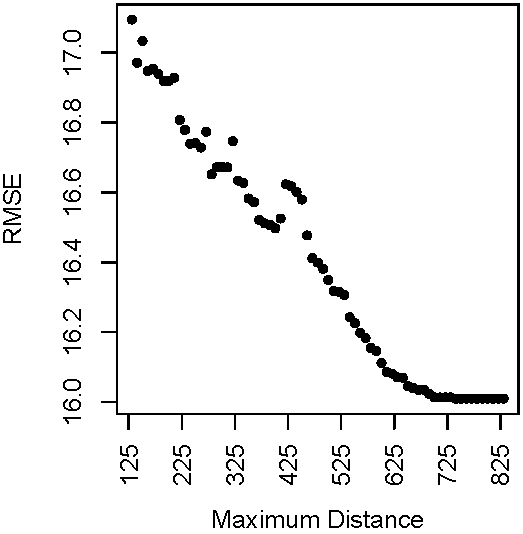
\includegraphics[width=\linewidth, keepaspectratio]{dismax.pdf}
\caption{Discharge}
\end{subfigure} \hspace{0.1\textwidth} %
\begin{subfigure}[t]{0.4\textwidth}
\centering
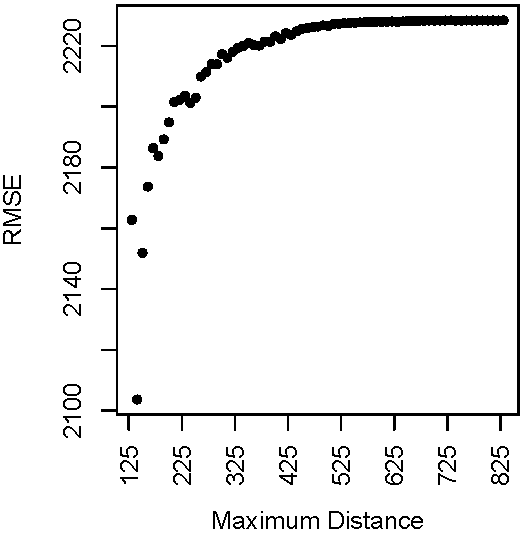
\includegraphics[width=\linewidth,, keepaspectratio]{salmax.pdf}
\caption{Salinity}
\end{subfigure}
\begin{subfigure}[t]{0.4\textwidth}
\centering
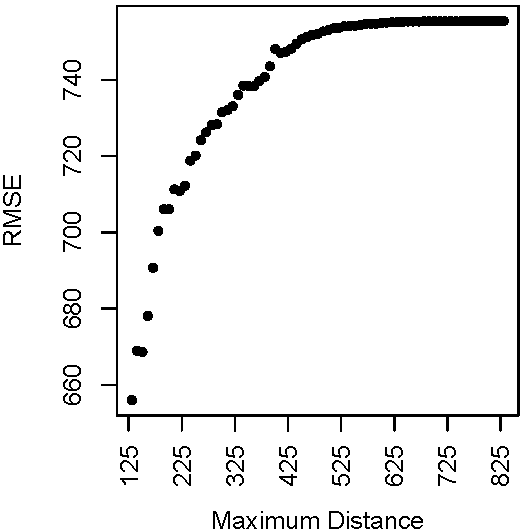
\includegraphics[width=\linewidth, keepaspectratio]{sedmax.pdf}
\caption{Sediment}
\end{subfigure} \hspace{0.1\textwidth} %
\begin{subfigure}[t]{0.4\textwidth}
\centering
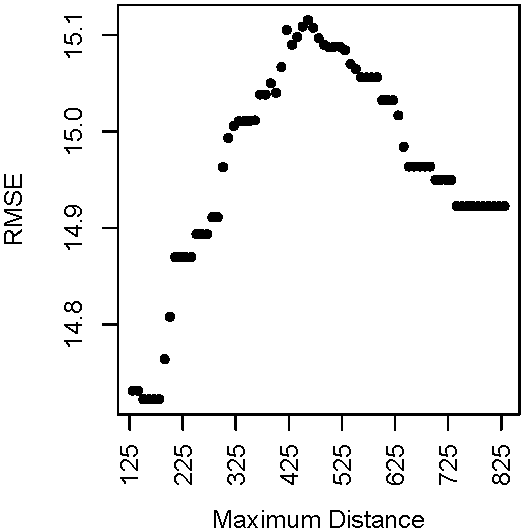
\includegraphics[width=\linewidth, keepaspectratio]{wlmax.pdf}
\caption{Water Level}
\end{subfigure}
\caption{The Alteration of RMSE Values with Increasing Maximum Distance for Discharge, Sediment, Salinity and Water Level}
\label{rmsemd}
\vspace*{-0.3cm}
\end{figure*}
% Please add the following required packages to your document preamble:
% \usepackage{multirow}
% \usepackage{graphicx}
\begin{table*}[!ht]
\centering
\caption{Descriptive Statistics (Minimum, Maximum, Mean and Standard Deviation) of the Data}
\label{descstat}
\resizebox{\textwidth}{!}{%
\begin{threeparttable}
\begin{tabular}{|l|l|l|l|l|l|l|}
\hline
\textbf{Type}               & \textbf{Predictor Class}                  & \textbf{Name}                                   & \textbf{Min} & \textbf{Max} & \textbf{Mean} & $\bm{\sigma^{2}}$ \\ \hline
\multirow{27}{*}{Predictor} & \multirow{7}{*}{Economic}                 & Having Own Land                                 & 0.937            & 1                & 0.982         & 0.017                       \\ \cline{3-7} 
                            &                                           & Having Pucca House\tnote{*}                          & 0.017            & 1.971            & 0.498         & 0.364                       \\ \cline{3-7} 
                            &                                           & House Ownership Ratio                           & 6.765            & 770.32          & 225.22       & 236.15                      \\ \cline{3-7} 
                            &                                           & 5 Acres+ Operated land                           & 0.084            & 50.29           & 4.938         & 9.855                       \\ \cline{3-7} 
                            &                                           & Income Source Business                          & 0.081            & 0.311            & 0.145         & 0.048                       \\ \cline{3-7} 
                            &                                           & Income Source Agriculture                       & 0.182            & 0.616            & 0.384         & 0.1                         \\ \cline{3-7} 
                            &                                           & Income Per Household Member                     & 0.023            & 0.837            & 0.048         & 0.101                       \\ \cline{2-7} 
                            & \multirow{6}{*}{Lifestyle}                & Household Size\tnote{*}                                  & 3.91             & 5.86             & 4.655         & 0.412                       \\ \cline{3-7} 
                            &                                           & Household Head Male                             & 5.71             & 36.74           & 19.34        & 7.885                       \\ \cline{3-7} 
                            &                                           & Households Using Tube Well and Supply Water                & 0.347            & 0.999            & 0.845         & 0.22                        \\ \cline{3-7} 
                            &                                           & Households Using Natural Water Sources                    & 0                & 0.377            & 0.036         & 0.084                       \\ \cline{3-7} 
                            &                                           & Households Using Other Water Sources            & 0                & 0.068            & 0.008         & 0.015                       \\ \cline{2-7} 
                            & \multirow{4}{*}{Educational}              & Male Literacy Rate\tnote{*}                              & 0.464            & 0.765            & 0.624         & 0.069                       \\ \cline{3-7} 
                            &                                           & Literacy Rate S.S.C/ H.S.C\tnote{*}                      & 0.043            & 0.169            & 0.091         & 0.027                       \\ \cline{3-7} 
                            &                                           & Literacy Rate Grad and Above                    & 0.004            & 0.027            & 0.012         & 0.006                       \\ \cline{3-7} 
                            &                                           & Literacy Rate                                   & 34.98            & 70.54            & 50.17        & 7.651                       \\ \cline{2-7} 
                            & \multirow{5}{*}{Environmental and Hydrologic}            & Low Land\tnote{*}                                        & 0                & 72               & 21.719        & 19.394                      \\ \cline{3-7} 
                            &                                           & River Length (miles)\tnote{*}                            & 15               & 180              & 71.189        & 32.863                      \\ \cline{3-7} 
                            &                                           & Rainfall (mm)\tnote{*}                                   & 90               & 344              & 180.484       & 46.83                       \\ \cline{3-7} 
                            &                                           & Humidity\tnote{*}                                        & 62.458           & 80.331           & 71.812        & 4.504                       \\ \cline{3-7} 
                            &                                             & Water Level\tnote{*}                                       & 1.37          & 90.81     & 16.146     & 16.654                        \\ \cline{3-7} 
                             &                                           & Discharge                                     & 2.7        & 83.3     & 11.692     & 12.574                                            \\ \cline{3-7} 
                            &                                           & Salinity                                      & 115.577        & 5287.659    & 1357.66     & 1829.731                                           \\ \cline{3-7} 
                            &                                           & Sediment\tnote{*}                                                  & 106.98       & 1539.12   & 736.2037     & 487.0911                                                                                                                                                                   \\ \cline{2-7} 
                            & \multirow{5}{*}{Precaution and Awareness} & Households Having Climate Change Knowledge      & 0.444            & 0.988            & 0.821         & 0.112                       \\ \cline{3-7} 
                            &                                           & Households Having Disaster Management Knowledge\tnote{*} & 0.099            & 6.816            & 1.767         & 1.112                       \\ \cline{3-7} 
                            &                                           & Households Having Sea Level Rise Awareness\tnote{*}      & 0.068            & 0.662            & 0.301         & 0.155                       \\ \cline{3-7} 
                            &                                           & Households Having Flood Awareness\tnote{*}               & 0.009            & 0.41             & 0.171         & 0.091                       \\ \cline{3-7} 
                            &                                           & Preparedness\tnote{*}                                    & 0                & 0.958            & 0.3           & 0.301                       \\ \hline
Response                    &                                           & Ratio of Total Affected Household               & 0                & 0.86             & 0.335         & 0.268                       \\ \hline

\end{tabular}%
\begin{tablenotes}
            \item[*] Significant predictors
\end{tablenotes}
\end{threeparttable}
}

\end{table*}
Among the predictors, water level, discharge, salinity and sediment had missing data. This is because stations for collecting these have not yet been constructed in every district. Out of 64 districts, stations measure discharge in 49, water level in 63, salinity in 29 and sediment in 15 districts. We estimate the missing data by following the Inverse Distance Weighting (IDW) interpolation technique. IDW has been used successfully in the literature to estimate missing data values of attributes such as rainfall \cite{chen2012estimation}. IDW assumes that the nearby points contribute more than the distant ones. According to IDW, the missing values are estimated using Equation \ref{IDW}.   
\begin{equation} \label{IDW}
\hat{x}=\sum_{i=1}^{n} w_{i}x_{i}
\end{equation}
Equation \ref{IDWW} shows how the the weight $w_{i}$ is calculated. 
\begin{equation} \label{IDWW}
w_{i}= \frac{d^{\gamma}_{i}}{\sum_{k=1}^{n} d^{\gamma}_{k}}
\end{equation}
Here, $x_{i}$ is the value of the predictor for nearby districts and $w_{i}$ is the weight calculated from Equation \ref{IDWW} and $d_{i}$ is the distance from each nearby district. Two parameters need to be specified for IDW which are the size of the neighborhood $n$ and the value of $\gamma$. In our experiments, we empirically selected $\gamma$ as 2. In case of neighborhood selection, some authors suggest to select a fixed number of nearby districts \cite{zimmerman1999experimental}. Another technique is to choose neighbors within a prespecified maximum distance. In our work, the maximum distance is selected as follows. We partition the data into two sets which are the data set with unknown values, $S_{u}$ and known values, $S_{k}$. The distances inside the range $(d_{min},d_{max})$ of $S_{k}$ are selected one by one as the maximum distance for neighborhood construction. For each maximum distance, IDW is utilized to estimate the missing values in $S_{u}$. These estimated values are used to further estimate the values of $S_{k}$ which are compared to its known values by RMSE. The maximum distance with the lowest RMSE is selected for defining the neighborhood. Figure \ref{rmsemd} shows the RMSE values for different maximum distance selection. The pattern of the alteration of RMSE depends on the data and the missing values. Hence, it is different for each of the predictors. From the figure, RMSE is lowest for discharge at 741, for salinity at 131, for sediment at 131 and for water level at 151.     

Table \ref{descstat} shows the mean, standard deviation, minimum and maximum values of the data. House ownership ratio, 5 Acres+ operated land, household head male, households using natural water sources and other water sources, low Land, river length (miles), water level, discharge, salinity, sediment and preparedness have comparatively larger standard deviation regarding their range. This increases the risk of non-normality of these predictors. However, In Section \ref{ttest}, it is showed that after transforming the predictors that exhibit non-linear relationship with the response, the normality assumption is satisfied.

\begin{figure}[ht!]
\centering
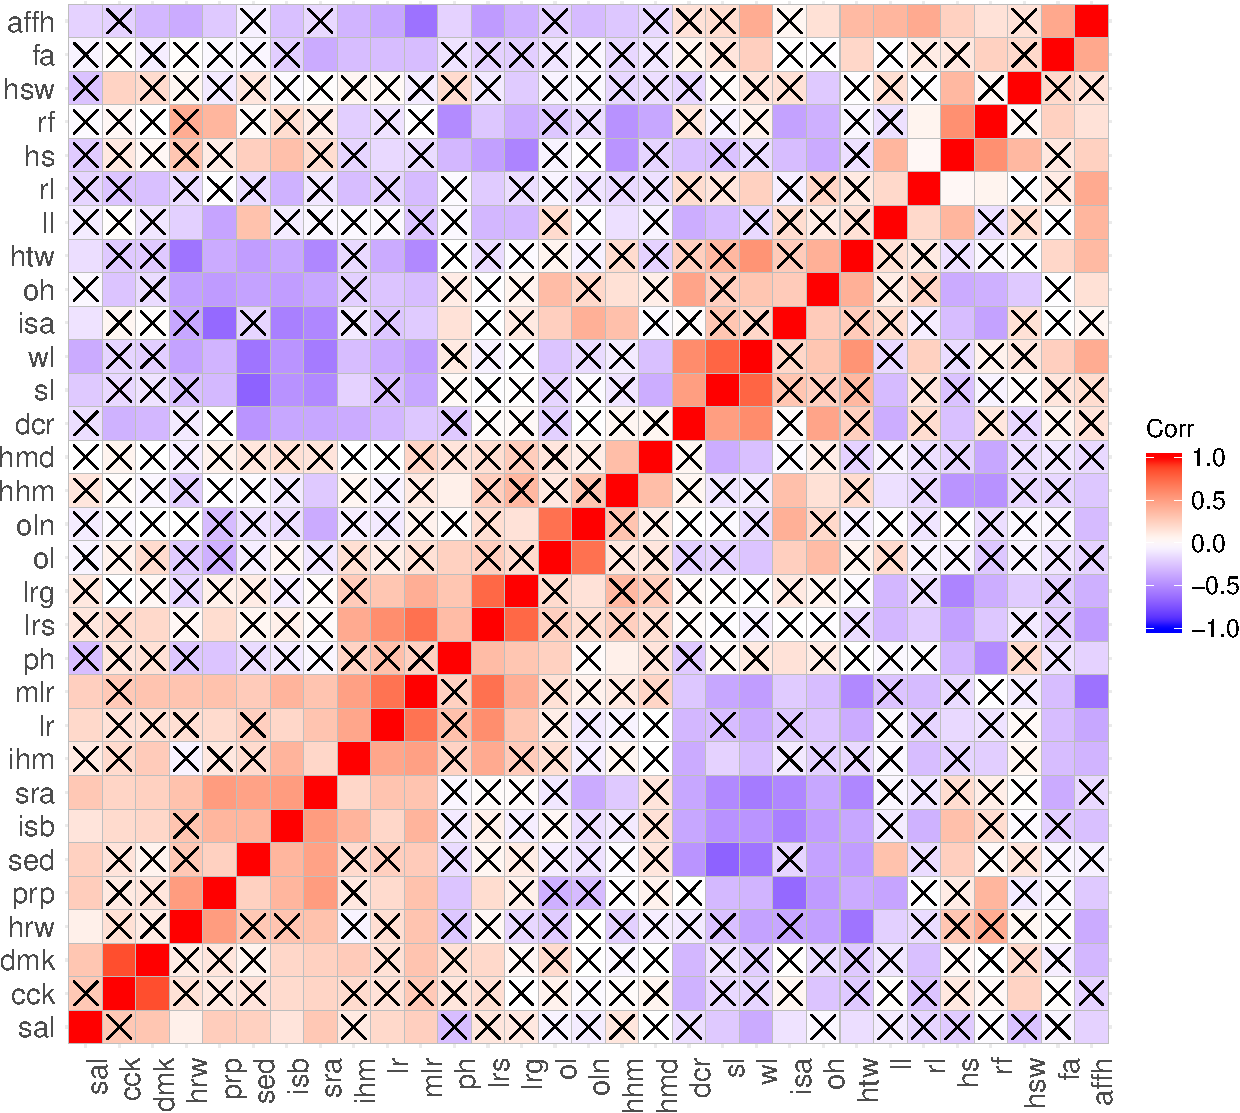
\includegraphics[width=90mm,keepaspectratio]{correlationplot.pdf}
\caption{Spearman's Rank Correlation of the Features at 0.1 Significance Level (Non-Significant Features are Marked with a Cross (X))}
\label{cor}
\end{figure}
Figure \ref{cor} depicts the Spearman's Rank Correlation values of the variables. Each cell depicts the correlation between the variables that form the cell. The non-significant predictors are crossed. For the ratio of total affected household, 14 features are statistically significant at 0.1 confidence level. Among these, male literacy (mlr) has the highest correlation value (-0.61) followed by households having flood awareness (fa) (0.45), river length (rl) (0.44), water level (wl) (0.43), literacy rate S.S.C/ H.S.C  (-0.43), literacy rate (lr) (-0.38), low land (ll) (0.38), households using natural water sources (hnw) (-0.36), households using tube well and supply water (htw) (0.35), literacy rate grad and above (lrg) (-0.34), income per household member (ihm) (-0.32), households having disaster management knowledge (dmk) (-0.31), 5 acres+ operated land (oln) (-0.29) and Income Source Business (isb) (-0.27). The correlation coefficients of some predictors are counterintuitive. For instance, salinity and sediment are negatively correlated with flood damage. Moreover, some important predictors do not show significant correlation. These issues occur due to two reasons. The first issue is data quality, for example, the hydrologic predictors had missing values and required to be imputed. Secondly, correlation does not consider the effect of other predictors opposed to multiple regression. A predictor may become significant when other predictors are held constant which is captured by multivariate regression. For example, Section \ref{rga} shows that these predictors are associated with the damage in an intuitive way. Along with the Spearman's Rank Correlation values, the Pearson correlation coefficient values were calculated and compared to the Spearman's correlation values. It was observed that both of these correlation values lie very close for most of the predictors. However, the Spearman's correlation values for 17 predictors are greater than Pearson correlation values. Out of these 17 predictors, 7 predictors are part of the selected features. Therefore, some of the selected features have a non-linear relationship with the response. As Random forest and multilayer perceptron models are non-parametric, this nonlinearity does not affect their performance. Nevertheless, as linearity is one of the assumptions of linear regression, data is transformed to satisfy this assumption (Section \ref{ttest}).

\begin{table}[!ht]
\centering
\footnotesize
\caption{MAE, RMSE and Correlation Coefficient values (* indicates statistically significant at 0.05 level compared to Linear Regression)}
\label{exp_tab}
\resizebox{90mm}{!}{%
\begin{tabular}{|p{1.8cm}|p{1.8425cm}|p{1.4cm}|p{2cm}|}
\hline
\textbf{Metrics}        & \textbf{Linear \newline Regression} & \textbf{Random Forest} & \textbf{Multilayer Perceptron} \\ \hline
MAE                     & 0.13                       & 0.16*                           & 0.22*                   \\ \hline
RMSE                    & 0.15                       & 0.20*                           & 0.28*                   \\ \hline
Correlation Coefficient & 0.80                        & 0.67*                           & 0.61                   \\ \hline
\end{tabular}%
}
\end{table}
\section{Result Analysis and Discussion}
\subsection{Paired T-Test}
\label{ttest}
Prior to the Paired T-Test, feature selection was performed following stepwise selection technique with AIC (Section \ref{method}). 14 features are selected which are shown in Table \ref{descstat}. After feature selection, the data is checked for linear regression assumptions and appropriate measures are applied when an assumption is violated. For example, Tukey's transformation is applied to improve the linearity of the predictors. The data is further standardized as mentioned in Section \ref{method}. A paired T-Test with linear regression as the base predictor is executed using this data. Table \ref{exp_tab} shows the Paired T-Test result of linear regression, multilayer perceptron and random forest at 0.05 confidence level. The RMSE values are 0.15, 0.20 and 0.28 for linear regression, random forest and multilayer perceptron respectively where 0.20 and 0.28 are significantly larger compared to linear regression. Similarly, for MAE, linear regression produces significantly better results than the other two. For correlation coefficient, linear regression performs significantly better than the other two. Therefore, the parametric model, linear regression is chosen for better explainability with acceptable prediction power. 

In previous studies such as \cite{poussin2014factors},  \cite{wagenaar2017multi} and \cite{dawson2008attribution}, linear regression was used without considering the six assumptions mentioned previously. As a result, Wagenaar et al. and Dawson et al. found linear regression to be outperformed by regression trees. The performance of a machine learning algorithm is highly dependent on predictor selection and preprocessing applied on data. Nevertheless, in our study, we ensure that the six assumptions are met for linear regression. Hence, the performance indicator values are more valid ones than those of previous studies. The linear regression assumptions are inspected and met as follows.

\begin{figure*}[!htp]
\centering
\begin{subfigure}[t]{0.23\textwidth}
\centering
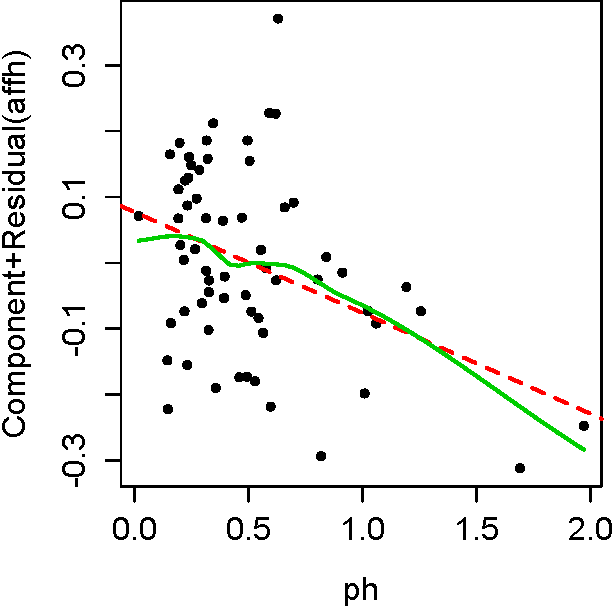
\includegraphics[width=\linewidth, keepaspectratio]{ph.pdf}
\caption{Having Pucca House}
\end{subfigure}
\begin{subfigure}[t]{0.23\textwidth}
\centering
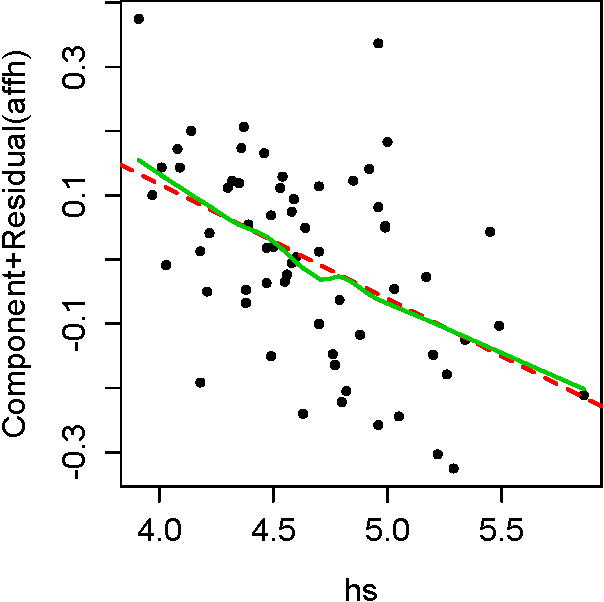
\includegraphics[width=\linewidth, keepaspectratio]{hs.pdf}
\caption{Household Size}
\end{subfigure}
\begin{subfigure}[t]{0.23\textwidth}
\centering
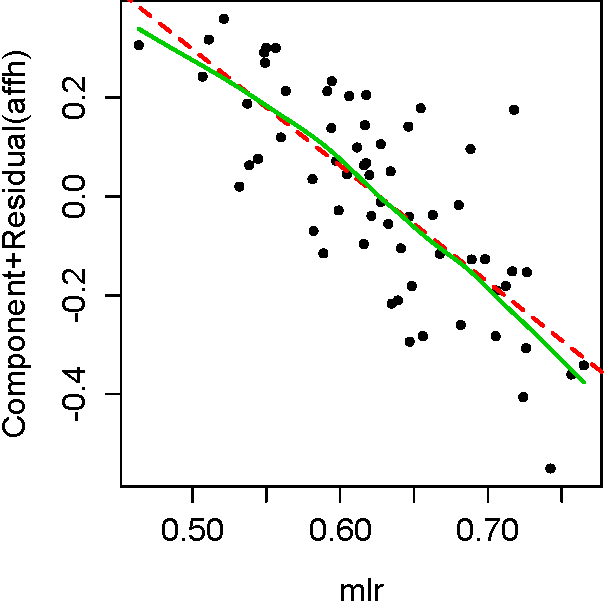
\includegraphics[width=\linewidth, keepaspectratio]{mlr.pdf}
\caption{Male Literacy Rate}
\end{subfigure}
\begin{subfigure}[t]{0.23\textwidth}
\centering
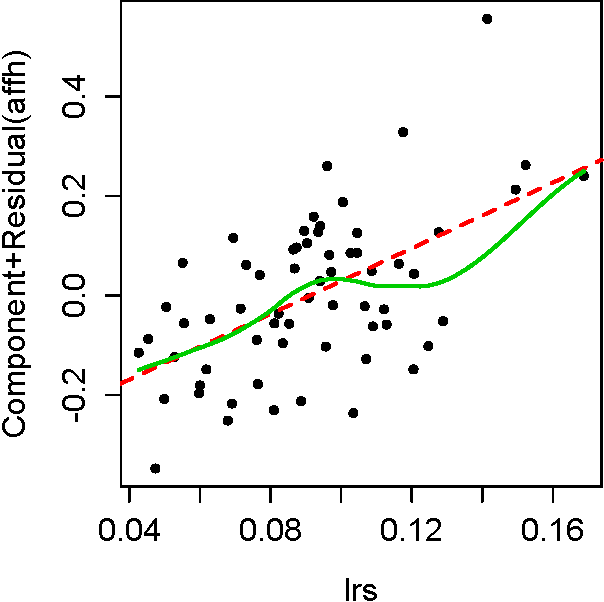
\includegraphics[width=\linewidth, keepaspectratio]{lrs.pdf}
\caption{Literacy Rate S.S.C / H.S.C}
\end{subfigure}
\begin{subfigure}[t]{0.23\textwidth}
\centering
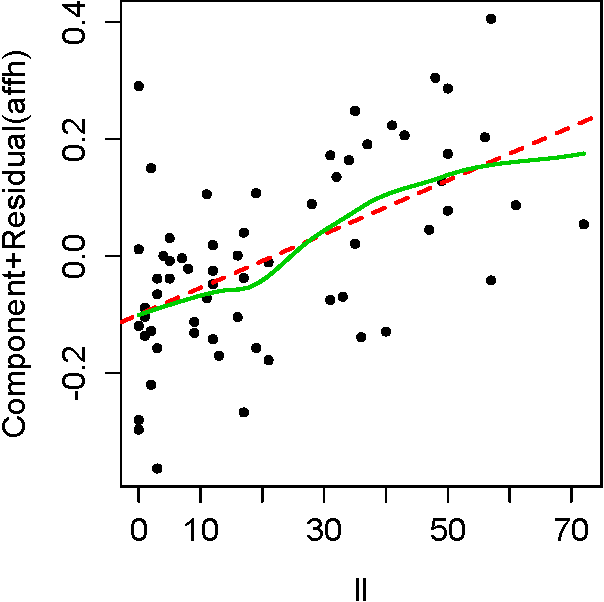
\includegraphics[width=\linewidth, keepaspectratio]{ll.pdf}
\caption{Low Land}
\end{subfigure}
\begin{subfigure}[t]{0.23\textwidth}
\centering
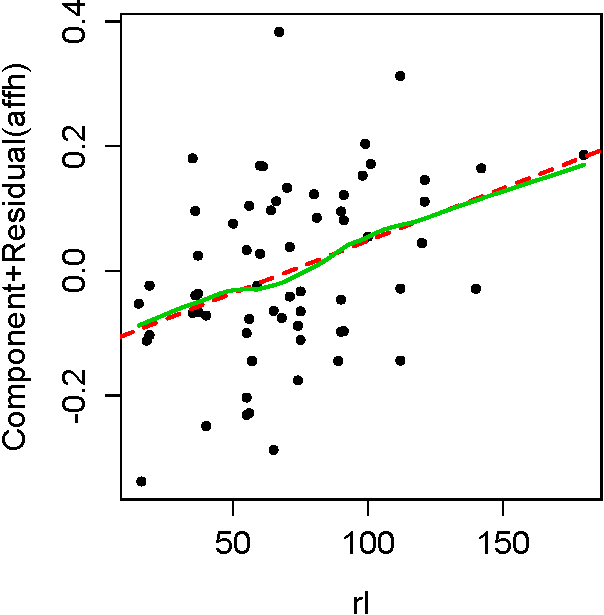
\includegraphics[width=\linewidth, keepaspectratio]{rl.pdf}
\caption{River Length}
\end{subfigure}
\begin{subfigure}[t]{0.23\textwidth}
\centering
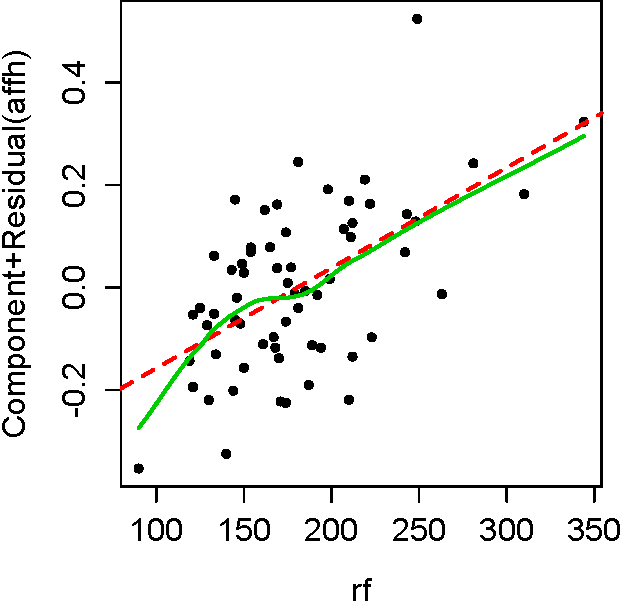
\includegraphics[width=\linewidth, keepaspectratio]{rf.pdf}
\caption{Rainfall}
\end{subfigure}
\begin{subfigure}[t]{0.23\textwidth}
\centering
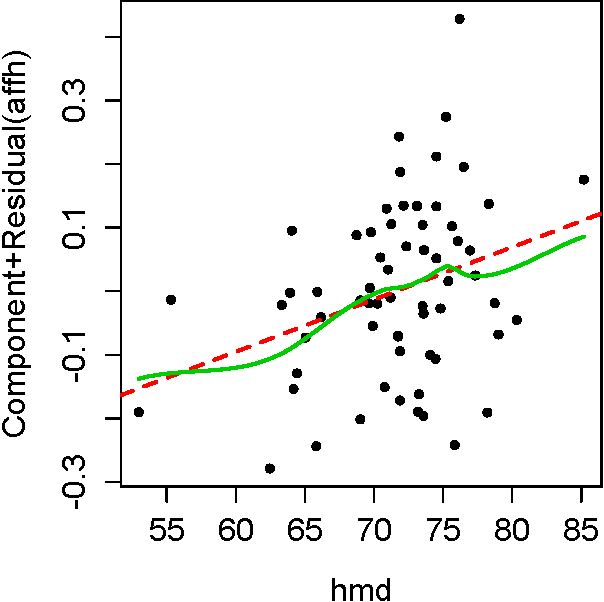
\includegraphics[width=\linewidth, keepaspectratio]{hmd.pdf}
\caption{Humidity}
\end{subfigure}
\begin{subfigure}[t]{0.23\textwidth}
\centering
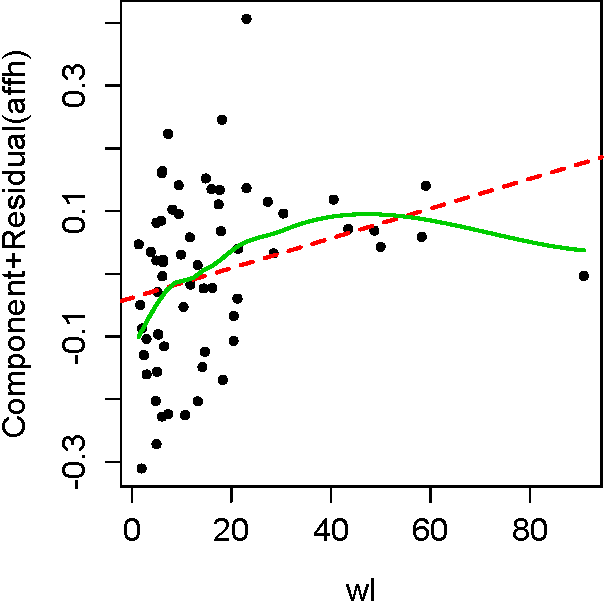
\includegraphics[width=\linewidth, keepaspectratio]{wl.pdf}
\caption{Water Level}
\end{subfigure}
\begin{subfigure}[t]{0.23\textwidth}
\centering
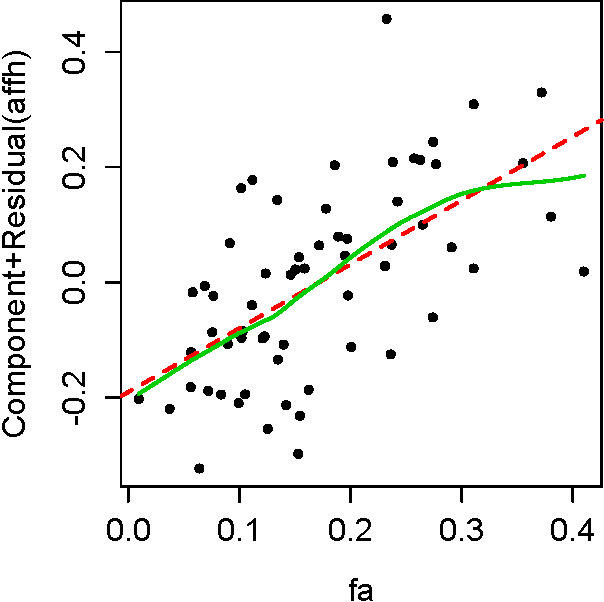
\includegraphics[width=\linewidth, keepaspectratio]{fa.pdf}
\caption{Households Having Flood Awareness}
\end{subfigure}\hspace{5mm}
\begin{subfigure}[t]{0.23\textwidth}
\centering
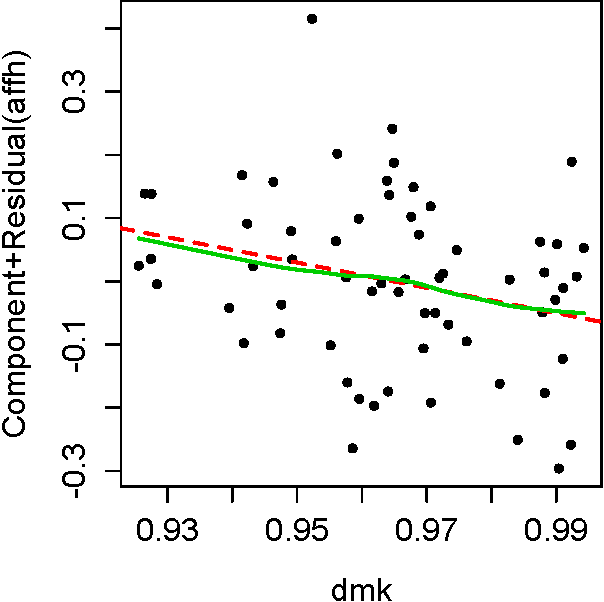
\includegraphics[width=\linewidth, keepaspectratio]{dmk.pdf}
\caption{Households Having Disaster Management Knowledge}
\end{subfigure}
\begin{subfigure}[t]{0.23\textwidth}
\centering
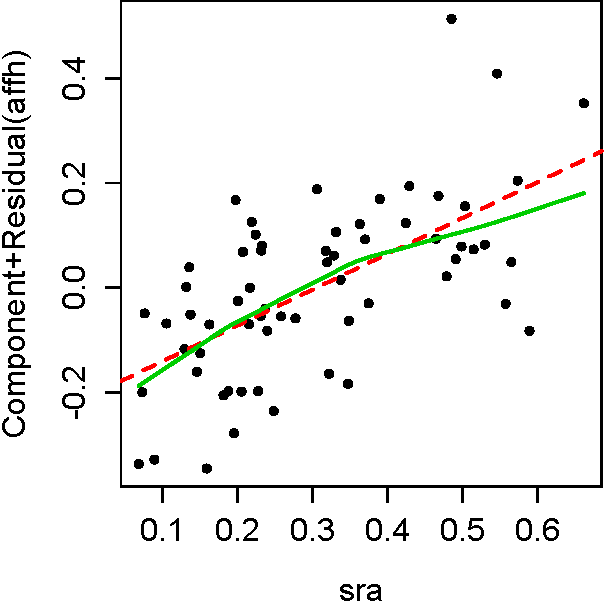
\includegraphics[width=\linewidth, keepaspectratio]{sra.pdf}
\caption{Households Having Sea Level Rise Awareness}
\end{subfigure}\hspace{5mm}
\begin{subfigure}[t]{0.23\textwidth}
\centering
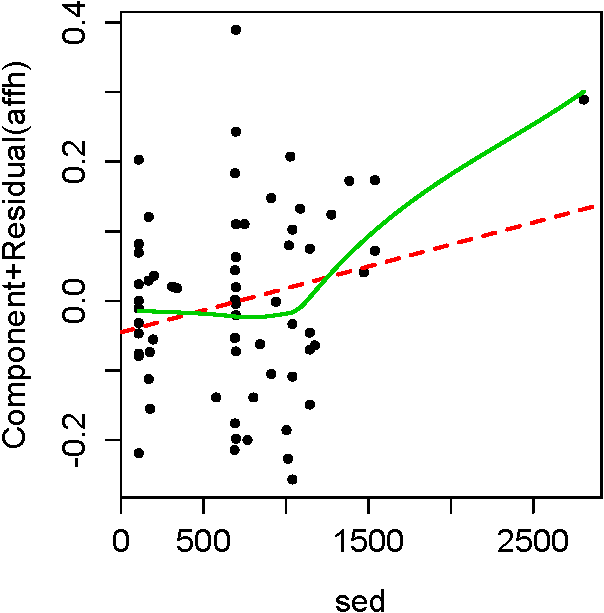
\includegraphics[width=\linewidth, keepaspectratio]{sed.pdf}
\caption{Sediment}
\end{subfigure}
\begin{subfigure}[t]{0.23\textwidth}
\centering
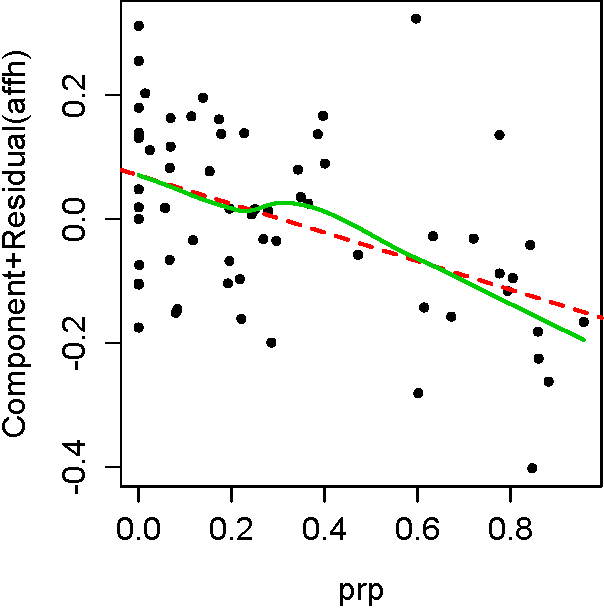
\includegraphics[width=\linewidth, keepaspectratio]{prp.pdf}
\caption{Preparedness}
\end{subfigure}
\caption{Component+Residual Plots for the Predictors (The Green Solid Line is the Partial Residual Line and the Red Dotted Line is the Linear Fit Line)}
\label{cr}
\vspace*{-0.3cm}
\end{figure*}
Although linearity assumption can be checked by plotting the predictors against the response, it does not consider the effect of a predictor with respect to the other predictors. In multivariate regression, the predictor-response relationship is assessed considering the presence of other predictors. Partial residual plots help to achieve this by plotting $residual+ \alpha_{i}x_{i}$ versus $x_{i}$ which is the green solid line in Figure \ref{cr}. The red dotted line is the linear fit line which represents a least squares regression line. Linearity assumption is verified by comparing how closely the first line lies to the least squares regression line. To improve the conformance to linearity assumption, the predictors can be transformed. This work uses the Tukey's power transformation where a linear model $y=a+bx$ is re-expressed as $y=a+bx^{\lambda}$ \cite{tukey1977exploratory}. The transformation is performed by continuously testing $\lambda$ with different values and observing whether the predictor-response relationship becomes linear. A series of $\lambda$ values can be tested using a table called Tukey's Ladder of Transformation \cite{tukey1977exploratory}. In this case, $\lambda = -2,-1,-\frac{1}{2},0,\frac{1}{2},1~\text{and}~2$ are used. Furthermore, $\lambda = 0$ is replaced by logarithmic transformation where $log(x)$ is used in place of $x$. We applied all the $\lambda$ values from the Tukey's Ladder of Transformation to all the predictor and examined linearity both graphically and quantitatively. Improved linearity was observed after transforming wl, sed, hmd, dmk, lrs and prp. Logarithmic transformation was applied to wl, dmk and hmd, and $\lambda=2$ was used for sed, lrs and prp. To say quantitatively, before applying the transformation, the values of $R^{2}$ and $\text{Adjusted}~R^{2}$ were 0.75 and 0.68 respectively. After transformation, $R^{2}$ and $\text{Adjusted}~R^{2}$ values increased to 0.8 and 0.74 respectively which indicates improved linearity.   

\begin{figure}[!ht]
\centering
    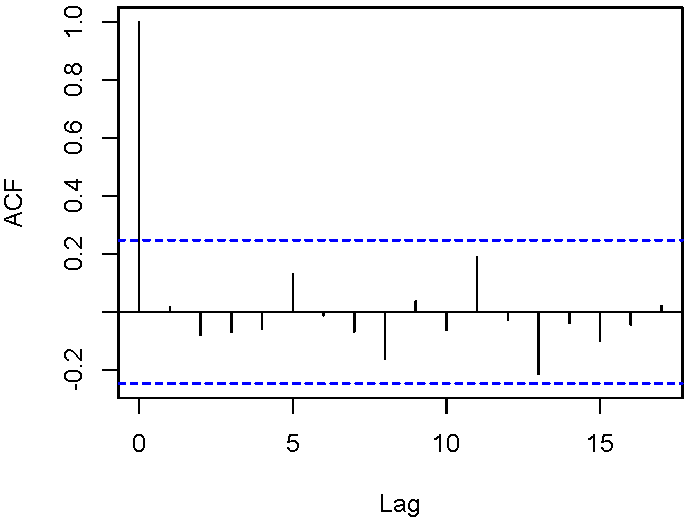
\includegraphics[width=90mm, keepaspectratio]{autocorrelation.pdf}
    \vspace{-0.2cm}
    \caption{Autocovariance and Autocorrelation Functions Plot (The Blue Dotted Lines Indicate 95\% Confidence Limits)}
    \label{afp}
\end{figure}
Figure \ref{afp} shows the autocorrelation function for residuals. The autocorrelation function measures the correlation among the residuals which can be expressed using Equation \ref{auto}.
\begin{equation}
F_{auto}=F_{cor}(r_{i},r_{i-n})
\label{auto}
\end{equation}
$F_{cor}$ measures the correlation between $i^{th}$ and $(i-n)^{th}$ residuals. The $n$ is the lag that represents the correlation between values in $n$ time periods distance. In the figure, the first vertical line with acf value 1 indicates the correlation of the residual with itself. The blue dotted lines are the 95\% confidence limits. If the values of the lags cross these lines, autocorrelation is present. From the figure, no autocorrelation is present as all the acf values of the lags (except lag 0) are within the confidence limits. This was further confirmed by Durbin-Watson test for autocorrelation \cite{durbin1951testing}. The p-value (0.2187) indicates that we cannot reject the null hypothesis of independence among residuals, that is, the residuals are not autocorrelated. 
\begin{figure}
  \centering
\begin{minipage}[!th]{0.45\textwidth}
\centering
   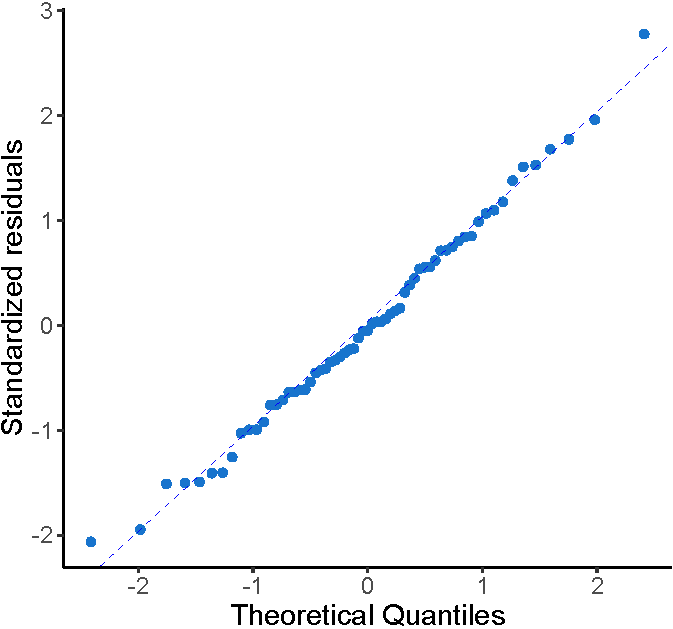
\includegraphics[width=45mm,keepaspectratio]{qqplot.pdf}
    \caption{Quantile-Quantile Plot}
     \label{diag}
\end{minipage}
\begin{minipage}[!th]{0.45\textwidth}\centering
   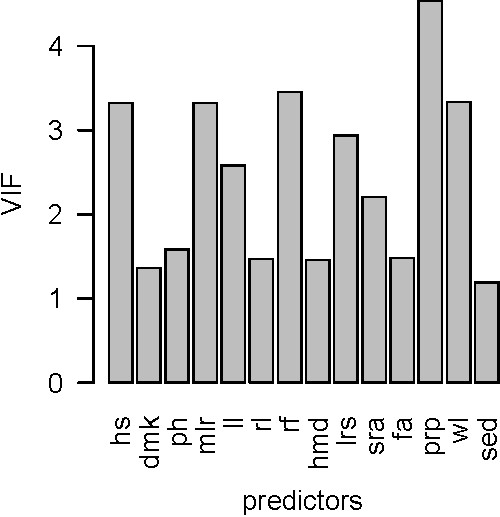
\includegraphics[width=45mm,keepaspectratio]{vif.pdf}
    \caption{VIF Plot}
     \label{vif}
\end{minipage}
\end{figure}

To detect heteroscedasticity, the Breush-Pagan test was conducted \cite{breusch1979simple}. Heteroscedasticity means that the variance of the residuals of a model is not equal across all the values of the response. The null hypothesis of the Breush-Pagan test is that the variances of the residuals are equal \cite{breusch1979simple}. The p-value of 0.6163 indicates that the null hypothesis cannot be rejected. Hence, heteroscedasticity is not present. For testing the normality assumption, the normal Q-Q plot is used which is shown in Figure \ref{diag}. The standardized residuals are plotted against quantiles of the standard normal distribution. The linear trend of the points indicates that the distribution of the residuals is approximately normal. This is further supported by a Shapiro-Wilk normality test where the null hypothesis is that the residuals come from a normally distributed population. The p-value of the test is 0.91. Therefore, the null hypothesis cannot be rejected. To examine multicollinearity, Variance Inflation Factor (VIF) is considered \cite{chatterjee1977regression}. Multicollinearity is the phenomenon when the predictor variables are intercorrelated. Multicollinearity is significant if VIF is greater than 10 \cite{chatterjee1977regression}. As Figure \ref{vif} depicts, VIF is less than 10 for all the predictors. Hence, multicollinearity is not significantly high. 
\begin{table}[!t]
\centering
\caption{Coefficients of Linear Regression Analysis (****p$<$0.001, ***p$<$0.01, **p$<$0.05, *p$<$0.1)}
\label{sigtab}
\resizebox{90mm}{!}{%
\begin{tabular}{|l|l|l|p{1.5cm}|p{1.2cm}|l|}
\hline
\textbf{Predictors}   & \textbf{Estimate} &\textbf{beta} & \textbf{Std. Error} & \textbf{\boldmath$T$ value} & \textbf{\boldmath$Pr(>|T|$)} \\ \hline
Intercept & 0.331****  &                           & 0.017      & 19.4    & \textless{}2E-16      \\ \hline
hs          & -0.080**   & -0.3                      & 0.031      & -2.6    & 0.013                 \\ \hline
dmk         & -0.037*    & -0.14                     & 0.02       & -1.9    & 0.067                 \\ \hline
ph          & -0.061***  & -0.23                     & 0.022      & -2.8    & 0.007                 \\ \hline
mlr         & -0.118**** & -0.44                     & 0.031      & -3.8    & 4.00E-04              \\ \hline
ll          & 0.099****  & 0.37                      & 0.028      & 3.6     & 7.00E-04              \\ \hline
rl          & 0.048**    & 0.18                      & 0.021      & 2.3     & 0.026                 \\ \hline
rf          & 0.080**    & 0.3                       & 0.032      & 2.5     & 0.016                 \\ \hline
hmd         & 0.056***   & 0.21                      & 0.021      & 2.7     & 0.01                  \\ \hline
lrs         & 0.062**    & 0.23                      & 0.029      & 2.1     & 0.041                 \\ \hline
sra         & 0.118****  & 0.44                      & 0.025      & 4.6     & 3.00E-05              \\ \hline
fa          & 0.102****  & 0.38                      & 0.021      & 4.9     & 1.00E-05              \\ \hline
prp         & -0.053     & -0.2                      & 0.036      & -1.4    & 0.157                 \\ \hline
wl          & 0.084***   & 0.32                      & 0.031      & 2.7     & 0.01                  \\ \hline
sed         & 0.047**    & 0.18                      & 0.019      & 2.5     & 0.016                 \\ \hline
\end{tabular}%
}
\end{table}
\subsection{Regression Analysis}
\label{rga}
As discussed previously, the data was fit to a linear regression model. To evaluate the model, cross-validation was performed. The $R^{2}$ and $\text{Adjusted}~R^{2}$ are 0.8 and 0.74 which indicates data fits well to the linear model. The F-Statistic is 13.77 on 14 and 48 degrees of freedom. The p-value of the F-Test is $2.589\mathrm{e}{-12}$ which is much less than the 0.05 significance level. This p-value signifies that the null hypothesis, the fit of the intercept-only model (the model without any predictors) and the fitted model is equal, can be rejected. 

Table \ref{sigtab} shows the regression analysis results. The estimate column contains the coefficient values. These are standardized for comparability which constitute the beta column. For significance level 0.001, 0.01, 0.05 and 0.1, the probability of observing any value larger than T is calculated. At 0.001 significance level, male literacy rate (mlr), sea level rise awareness (sra), flood awareness (fa) and low land (ll) predictors are related to the response. The negative slope of mlr indicates that increasing male literacy rate contributes to decreasing damage. To further analyze the effect of gender and literacy on damage, we replaced male literacy with female literacy rate and re-conducted the analysis. The female literacy rate was observed to be negatively related to damage at 0.001 significance level with a standardized coefficient of -0.478. We inspected whether there is a statistically significant difference between the standardized regression coefficient of male and female literacy. To do this, a boolean indicator called f (0 for male and 1 for female) and an interaction term $\text{f} \times \text{lrmf}$ were included as predictors, where lrmf indicates literacy rate of male or female. Equation \ref{fem} and \ref{femcase} show that the coefficient of the interaction term $\alpha_{3}$ captures the difference between the coefficients of male and female literacy.
\begin{equation}
\begin{split}
affh=\alpha_{1} \times f + \alpha_{2} \times lrmf+ \alpha_{3} \times f \times lrmf+\\
\alpha_{4} \times hs + \cdots + c 
\label{fem}
\end{split}
\end{equation}
\begin{equation}
affh= 
\begin{dcases}
(\alpha_{2}+\alpha_{3}) \times lrmf+\alpha_{4} \times hs \\
+\cdots + c+\alpha_{1}
, & f=1 \\
\alpha_{2} \times lrmf+ \alpha_{4} \times hs + \cdots + c , & f=0 \\
\end{dcases}
\label{femcase}
\end{equation}
A regression analysis was performed including these predictors where $\alpha_{3}$ was observed to be statistically insignificant. Therefore, there is no statistically significant difference between the contribution of male and female literacy on damage risk reduction. The finding that literacy reduces damage is consistent with the findings by Thieken et al., poussin et al. and Merz et al. \cite{thieken2005flood, poussin2014factors, merz2013multi}. Thieken et al. and Merz et al. showed that higher socio-economic status by Plapp \cite{plapp2004wahrnehmung}, decided by education, job position, income etc., is correlated with lower damage \cite{thieken2005flood, merz2013multi}. Poussin et al. showed that education is positively associated with avoidance measures.    

Districts with more low lands face more flood damage as indicated by the positive coefficient of ll. According to the coefficients of fa and sra, an increase of these variables results in increased damage. This counter-intuitive scenario happens because people in disaster-prone areas have higher flood and sea-level awareness through experiencing disasters over time. To examine this, we extracted the subset of highly affected households determined by affh values greater than the upper quartile. The regression analysis was rerun with this data. It was seen that both fa and sra were negatively related to affh (not shown here). The predictor fa is associated with flood experience and flood knowledge. According to Thieken et al., Poussin et al. and Bubeck et al, knowledge on flood hazard and experience are significantly related to reduced flood damage, which is confirmed by the high significance of fa in our study.  

\begin{figure}[!ht]
  \centering
    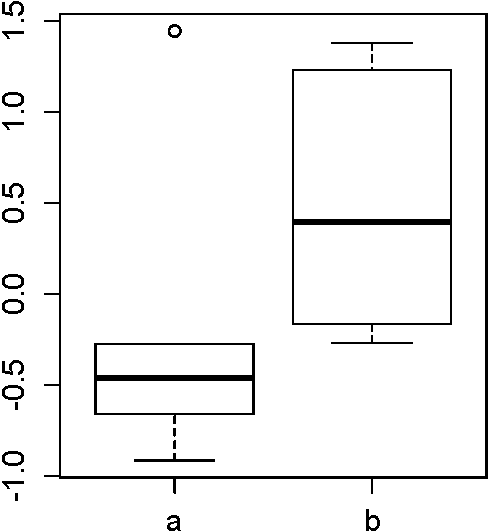
\includegraphics[width=60mm, keepaspectratio]{boxplotprp.pdf}
    \caption{Distribution of the households having disaster management knowledge on two scenario- (a) high damage and preparedness (b) low damage and preparedness}
    \label{boxp}
\end{figure}
At 0.01 and 0.05 confidence level, household size (hs), having pucca house (ph), river length (rl), rainfall (rf), humidity (hmd), water level (wl), sediment (sed) and literacy rate S.S.C/ H.S.C (lrs) are related to the damage. Larger households leads to lower flood damage. This is because household size positively influences precaution measures \cite{thieken2007coping}. The ownership of a pucca house is positively related to damage similar to the literature \cite{zhai2005modeling,kreibich2005flood}. The environmental and hydrologic components namely rainfall, water level, sediment and humidity positively influence flood damage. Flood damage intensifies with increasing lrs. However, the literacy rate of grad and above (lrg) is negatively correlated with flood affected households when it is fitted to a regression model with affh as response (not shown here). Hence, lrs can be regarded as lack of higher education. These results regarding lrs and lrg corresponds to the issue that higher education level is associated with lower flood damage risk which is supported by the literature \cite{islam2012coping}. Preparedness is considered to be an important factor in the literature \cite{thieken2005flood,merz2013multi} which is, however, statistically insignificant in our analysis. This is because preparedness, which is the act of taking action regarding flood, is effective when it is supported by disaster management knowledge. This is explained using Figure \ref{boxp} which shows the distribution of disaster management knowledge when (a) preparedness and damage is high and (b) preparedness and damage is low. Here, high and low correspond to the upper and lower quartiles respectively. In scenario a, when preparedness is high, damage can be high if disaster management knowledge is low. In scenario b, damage is low although preparedness is low because the number of households with disaster management knowledge is higher than the previous scenario (Figure \ref{boxp}). In our analysis, disaster management knowledge is negatively associated with the ratio of total affected household. However, it is less significant than the other predictors. This is similar to the findings by Thieken et al. and Bubeck et al. \cite{thieken2005flood,bubeck2012long}.  
\begin{figure}[!ht]
  \centering
    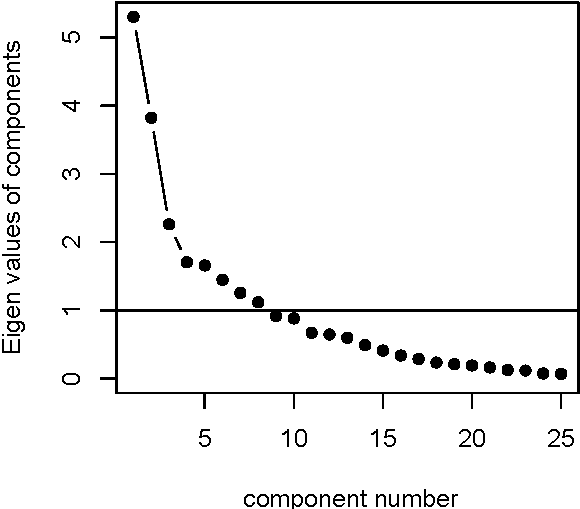
\includegraphics[height=7cm, keepaspectratio]{screePlot.pdf}
    \caption{Scree Plot for Principal Component Analysis}
    \label{scree}
\end{figure}
\begin{table*}[!th]
\centering
\footnotesize
\caption{Varimax Rotated Loading Vectors of First and Second Principal Components (Values with absolute loadings $\geq$ 0.5 are bolded)}
\label{pca}
\begin{tabular}{|l|l|l|l|l|l|l|l|l|}
\hline
\textbf{Variables} & \textbf{PC1}  & \textbf{PC2}   & \textbf{PC3}   & \textbf{PC4}   & \textbf{PC5}  & \textbf{PC6}   & \textbf{PC7}   & \textbf{PC8}   \\ \hline
ol        & 0.1           & -0.1          & 0.03           & -0.05          & 0.12          & \textbf{0.84} & -0.1          & -0.11         \\ \hline
lr        & \textbf{0.73} & 0.19          & -0.12          & 0.13           & 0.02          & 0             & 0.09          & -0.36         \\ \hline
isb       & 0.03          & \textbf{0.76} & -0.03          & 0.09           & 0.15          & -0.01         & 0.12          & -0.09         \\ \hline
hs        & -0.39         & 0.27          & 0.04           & \textbf{0.7}   & 0.11          & 0.15          & 0.23          & 0.1           \\ \hline
ihm       & 0.44          & \textbf{0.51} & 0.13           & 0.03           & 0.22          & -0.11         & 0.12          & -0.21         \\ \hline
hhm       & -0.08         & -0.04         & 0.07           & \textbf{-0.86} & 0.04          & 0.14          & 0.11          & -0.04         \\ \hline
cck       & 0.03          & 0.07          & 0.05           & 0.02           & \textbf{0.91} & 0.02          & 0.12          & -0.04         \\ \hline
dmk       & 0.11          & 0.04          & -0.07          & 0.01           & \textbf{0.91} & 0.1           & -0.05         & 0.05          \\ \hline
ph        & 0.31          & -0.29         & 0.24           & -0.3           & 0.27          & 0.15          & -0.29         & \textbf{-0.5} \\ \hline
mlr       & \textbf{0.73} & 0.37          & -0.25          & -0.02          & 0.17          & 0.19          & 0.03          & -0.13         \\ \hline
ll        & -0.2          & -0.3          & 0.2            & 0.47           & 0.02          & 0.2           & \textbf{0.57} & -0.31         \\ \hline
rf        & -0.21         & 0.41          & -0.02          & \textbf{0.55}  & 0.07          & -0.02         & -0.09         & 0.38          \\ \hline
lrs       & \textbf{0.88} & 0.1           & -0.01          & -0.07          & 0.1           & 0.07          & -0.05         & 0.04          \\ \hline
lrg       & \textbf{0.73} & -0.19         & -0.11          & -0.34          & -0.04         & 0.04          & 0.08          & 0.12          \\ \hline
oln       & 0.14          & -0.09         & 0.06           & 0              & 0.04          & \textbf{0.7}  & 0.14          & 0.32          \\ \hline
isa       & -0.08         & \textbf{-0.8} & 0.01           & -0.26          & 0.05          & 0.24          & 0.1           & 0.03          \\ \hline
fa        & -0.1          & -0.11         & 0.11           & 0.12           & 0.03          & 0.06          & -0.04         & \textbf{0.79} \\ \hline
htw       & -0.14         & -0.19         & \textbf{0.89}  & 0.02           & -0.03         & -0.05         & -0.05         & 0.14          \\ \hline
hnw       & 0.04          & 0             & \textbf{-0.91} & 0.05           & -0.02         & -0.13         & -0.08         & 0.09          \\ \hline
prp       & 0.27          & \textbf{0.77} & -0.43          & -0.03          & 0.08          & 0.03          & 0.03          & -0.01         \\ \hline
wl        & -0.04         & -0.4          & \textbf{0.5}   & 0.03           & -0.06         & -0.37         & -0.34         & 0.31          \\ \hline
sed       & 0.11          & 0.08          & -0.04          & -0.08          & 0.06          & -0.06         & \textbf{0.87} & 0.03          \\ \hline
\end{tabular}

\end{table*}
\subsection{Principal Component Analysis}
To understand the grouped interaction of the variables on the flood damage, Principal Component Analysis (PCA) was performed. The number of significantprincipal components was chosen based on Kaiser criterion and the scree plot. According to Kaiser criterion, 8 principal components have been selected as seen from Figure \ref{scree}. These explain 72\% of the total variance. Table \ref{pca} shows the varimax rotated loadings of these principal components. Using a cut-off factor of 0.5, only the significant variables are shown where their loadings are marked as bold. The first component represents literacy with high positive loadings of literacy rate (lr), Male Literacy Rate (mlr), Literacy Rate S.S.C/ H.S.C (lrs) and Literacy Rate Grad and Above (lrg). The second component represents income with income source business (isb), income source agriculture (isa) and income per household member (ihm), and preparedness (prp). The third principal component captures the water level (wl) and source of drinking water (households using tube well and supply water (htw), and households using natural source of water (hnw)). The fourth one is related to household structure consisting of household size (hs) and household head male (hhm), and rainfall (rf). The fifth one consists of households having climate change knowledge (cck) and disaster management knowledge (dmk). The sixth principal component represents land ownership with positive loadings of having own land (ol) and 5 acres+ operated land (oln). The seventh one is related to low land (ll) and sediment (sed), and the eighth one represents house structure with a negative loading of having pucca house (ph), and flood awareness (fa). 

\begin{table}[!t]
\centering
\caption{Coefficients of Linear Regression Analysis with Principal Components (****p$<$0.001, ***p$<$0.01, **p$<$0.05, *p$<$0.1)}
\label{sigtabpca}
\resizebox{90mm}{!}{%
\begin{tabular}{|l|l|p{1.2cm}|l|l|}
\hline
\textbf{Predictors} & \textbf{Estimate} & \textbf{Std. Error} & \textbf{\boldmath$T$ value} & \textbf{\boldmath$Pr(>|T|$)} \\ \hline
Intercept           & 0.3912            & 0.0281              & 13.9             & 0                              \\ \hline
PC1                  & -0.0786***        & 0.0238              & -3.31            & 0.0017                         \\ \hline
PC2                  & -0.041*          & 0.0238              & -1.72            & 0.0906                         \\ \hline
PC3                  & 0.0899****        & 0.024               & 3.75             & 0.0004                         \\ \hline
PC4                  & 0.0653***         & 0.0238              & 2.74             & 0.0083                         \\ \hline
PC5                  & -0.0507**         & 0.0237              & -2.14            & 0.0373                         \\ \hline
PC6                  & -0.0616****       & 0.0157              & -3.94            & 0.0002                         \\ \hline
PC7                  & 0.0786***         & 0.0242              & 3.24             & 0.002                          \\ \hline
PC8                  & 0.0753***         & 0.0254              & 2.97             & 0.004                          \\ \hline
\end{tabular}%
}
\end{table}
Table \ref{sigtabpca} shows regression analysis results using the principal components as predictors and the ratio of total affected households (affh) as response. Considering the coefficient estimates and the Pr values, the principal components can be ranked as PC3, PC6, PC1, PC7, PC8, PC4, PC5 and PC2. Flood damage increases with PC1 indicating that increased water level and the use of tube well and supply water is associated with higher damage where the use of natural water sources is negatively related to damage. This is because from Figure \ref{cor} we observe that people in areas with high water level tend to use tube well and supply water more than natural sources of water. The negative coefficient of PC6 shows that higher amount of land ownership is related to lower flood damage. Higher literacy rate contributes to lower affected households as seen from the coefficient of PC1. The positive association between PC7 and affh is because ll and sed both are positively correlated with affh. For PC8, flood damage increases as ph and fa increase. The counter-intuitive case of positive association between affh and fa is due to the aforementioned reason (Section \ref{rga}). According to the positive coefficient of PC4, damage increases with increasing household size and rainfall, and decreasing male to female household head ratio. PC5 and PC2 are negatively related to affh. For PC5, it means higher disaster related knowledge (dmk and cck) leads to lower damage. In case of PC2, isb leads to better income and literacy (Figure \ref{cor}) resulting in decreased affh where isa indicates otherwise. Moreover, Higher preparedness is associated with lower damage. 

Hydrologic and environmental components with wl, sed, ll and rf variables show highly significant correlation with damage according to PC3, PC7 and PC4. PC3 is significant at 0.001, and PC7 and PC4 significant at 0.01 significance level. Variables that influence ownership and socio-economic status such as literacy (PC1), land ownership (PC6) and house structure (PC8) are highly significant for predicting affh (Table \ref{sigtabpca}). However, disaster knowledge (PC5) and preparedness (PC2) show comparatively less significance. These are consistent with the findings by Thieken et al. where loss ratio is significantly correlated with hydrologic and environment factors (flood impact items), ownership and socio-economic status, and less correlated with precaution and disaster knowledge related factors \cite{thieken2005flood}.        

\section{Conclusion}
This paper has derived a machine learning based model for flood damage analysis from district-level data of affected households. Most of the studies in the literature consider building-level damage and limited set of areas or floods. The paper differs as it adopts a higher spatial scale (households) and uses a 6-year flood data of 64 districts. Linear regression is the strongest prediction algorithm for this data with MAE 0.13, RMSE 0.15 and correlation coefficient 0.80. The findings from the regression analysis are mostly consistent with the literature. Inconsistencies occur in case of preparedness. According to our study, preparedness is effective in flood damage reduction when it is supported by disaster management knowledge. In addition, a few factors from PCA such as income per household member, household head male and source of drinking water show counter-intuitive behavior.

Some recommendations can be made from this study. Firstly, literacy is an important predictor of flood damage. The data shows that literacy rate degrades significantly from S.S.C/ H.S.C to higher education phase. This issue requires further attention. The importance of male and female literacy need to be considered equally. Secondly, preparedness is not enough for flood damage mitigation. Initiatives should be taken to both educate the people about disaster management before, during and after a disaster, and enable them to convert this knowledge into effective flood handling actions. As seen from the correlation coefficients, flood awareness is not significantly correlated with disaster management knowledge and preparedness. Therefore, the people who have experienced floods are required to be treated with equal attention regarding disaster management knowledge transfer and preparedness improvement.

\noindent 
%% References

\bibliographystyle{elsarticle-num}
\bibliography{IJDRR_references}

\end{document}

%%
%% End of file.
